%From https://egu2018.eu/PICO_how-to_guide_to_PICO.pdf
%Abstracted and templated by Brian Ballsun-Stanton, Macquarie University.
%original template by https://github.com/snowtechblog/pico-latex-presentation by Anselm Köhler

\documentclass[unknownkeysallowed,usepdftitle=false, parskip=full]{beamer}
% unknownkeysallowed is needed for mac and the newer latex version -> is more picky than before...
\usetheme[headheight=1cm,footheight=2cm]{boxes}
%\usetheme{default}


\usepackage{default}
\usepackage{graphicx}
\usepackage{hyperref}
%example pictures created via: http://lorempixel.com/1200/800/cats/Figure2/. Credit to http://lorempixel.com/images.php

\usepackage{epsfig}
\usepackage{siunitx}
\usepackage{color}
\usepackage{ifthen}
%usepackage{ragged2e}

\usepackage[T1]{fontenc}
\usepackage[utf8]{inputenc}
%https://tex.stackexchange.com/a/203804/5483

\usepackage[activate={true,nocompatibility},final,tracking=true,kerning=true,spacing=true,factor=1100,stretch=10,shrink=10]{microtype} % http://www.khirevich.com/latex/microtype/
\microtypecontext{spacing=nonfrench}

\usepackage{lipsum} % for dummy text only
\usepackage[UKenglish]{babel} %https://tex.stackexchange.com/a/27743 
\usepackage[pangram]{blindtext} % https://tex.stackexchange.com/a/48411

%\usepackage{parskip} % from https://tex.stackexchange.com/q/11622
%\setlength{\parskip}{12pt} 

%\setparsizes{\parindent}{12pt}{\parfillskip}

%\usepackage{etoolbox} % as per https://tex.stackexchange.com/a/24331
%\appto\chapterheadendvskip{\vspace{-1\parskip}}
%\setparsizes{\parindent}{50pt plus 20pt minus 30pt}{\parfillskip}

\setbeamertemplate{navigation symbols}{}%remove navigation symbols
\setbeamersize{text margin left=1cm,text margin right=1cm}

% some colors
\definecolor{grau}{gray}{.5}
\definecolor{slfcolor}{rgb}{0,0.6274,0.8353}
\definecolor{wslcolor}{rgb}{0,0.4,0.4}

% setup links
\hypersetup{%
	%linkbordercolor=green,%
	colorlinks=false,%
	pdfborderstyle={/S/U/W 0},%
	%pdfpagemode=FullScreen,%
	pdfstartpage=4%
	}

% setup some fonts
\setbeamerfont{title}{series=\bfseries, size=\small}
\setbeamerfont{author}{size*={5pt}{0pt}}
\setbeamerfont{institute}{size*={3pt}{0pt}}
\setbeamerfont{bodytext}{size=\scriptsize}
	
% Title setup	
\title{Conversion and Analysis From Multiple Data Sources}
\author{Aaron Hammond 1\inst{1} (\texttt{aaron.hammond1@students.mq.edu.au}) }
\institute{\inst{1}Macquarie University, Sydney, NSW}
% add title in headbox
\setbeamertemplate{headline}
{\leavevmode
\begin{beamercolorbox}[width=1\paperwidth]{head title}
  % LOGO
  \begin{columns}[t, totalwidth=\textwidth]
  \begin{column}[c]{1.05cm}
     
\includegraphics[width=1cm]{figure/ubuntu-logo32.png}
  \end{column}
  % TITLE
   \begin{column}[c]{10.6cm}
   \centering \usebeamerfont{title} \textcolor{slfcolor}{\inserttitle} \\
   \centering \usebeamerfont{author} \color[rgb]{0,0,0} \insertauthor \\
   \vspace{-0.05cm}
   \centering \usebeamerfont{institute} \insertinstitute
  \end{column}
  % PICTURE
  \begin{column}[c]{1.15cm}
    \hspace{0.005cm}
    
\includegraphics[width=1cm]{figure/voyantlogo.PNG}
  \end{column}
  \end{columns}
  {\color{slfcolor}\hrule height 1pt\vspace{0.1cm}}
\end{beamercolorbox}%
}

% setup the navigation in footbox
% first set some button colors
\newcommand{\buttonactive}{\setbeamercolor{button}{bg=wslcolor,fg=white}}
\newcommand{\buttonpassive}{\setbeamercolor{button}{bg=slfcolor,fg=black}}
% now set up that the one active one gets the new color.
\newcommand{\secvariable}{nothing}
% therefore we write before each section (well, everything which should be part of the navi bar)
% the variable \secvariable to any name which is in the next function ...
\newcommand{\mysection}[1]{\renewcommand{\secvariable}{#1}
}
% ... compaired to strings in the following navibar definition ...
\newcommand{\tocbuttoncolor}[1]{%
 \ifthenelse{\equal{\secvariable}{#1}}{%
    \buttonactive}{%
    \buttonpassive}
 }
% ... here we start to set up the navibar. each entry is calling first the function \tocbuttoncolor with the argument which should be tested for beeing active. if active, then change color. afterwards the button is draw. so to change that, you need to change the argument in \toc..color, the first in \hyperlink and before each frames definition... A bit messed up, but works...
\newlength{\buttonspacingfootline}
\setlength{\buttonspacingfootline}{-0.2cm}
\setbeamertemplate{footline}
{\leavevmode
\begin{beamercolorbox}[width=1\paperwidth]{head title}
  {\color{slfcolor}\hrule height 1pt}
  \vspace{0.05cm}
  % set up the buttons in an mbox
  \centering \mbox{
    \tocbuttoncolor{abstract}
    \hyperlink{abstract}{\beamerbutton{2 Minute Madness}}
    \tocbuttoncolor{radar}
    \hspace{\buttonspacingfootline}
      \hyperlink{radar}{\beamerbutton{Section 1}}

    \tocbuttoncolor{line}
    \hspace{\buttonspacingfootline}
      \hyperlink{line}{\beamerbutton{Section 2}}
    \tocbuttoncolor{major}
    \hspace{\buttonspacingfootline}
      \hyperlink{major}{\beamerbutton{Section 3}}
    \tocbuttoncolor{slab}
    \tocbuttoncolor{conclusion}
    \hspace{\buttonspacingfootline}
      \hyperlink{conclusion}{\beamerbutton{Conclusion}}
    % this last one should normaly not be used... it will open the preferences to change the 
    % behaviour of the acrobat reader in fullscreen -> usefull in pico...
    \setbeamercolor{button}{bg=white,fg=black}
    % for presentation
    %\hspace{-0.1cm}\Acrobatmenu{FullScreenPrefs}{\beamerbutton{\#}}
    % for upload
    
     
\Acrobatmenu{FullScreenPrefs}{\vspace{0.3cm}\hspace{0.24cm}\mbox{%
      
\includegraphics[height=0.04\textheight,keepaspectratio]{%
	  figure/CreativeCommons_Attribution_License.eps}%
	  }}
   }
    \vspace{0.05cm}
\end{beamercolorbox}%
}


\begin{document}


%%%%%%%%%%%%%%%%%%%%%%%%%%%%%%%%%%%%%%%%%%%%%%%%%%%%%%%%%%%%%%%%%%%%%%%%%%
\mysection{abstract}
%%%%%%%%%%%%%%%%%%%%%%%%%%%%%%%%%%%%%%%%%%%%%%%%%%%%%%%%%%%%%%%%%%%%%%%%%%
\begin{frame}\label{\secvariable}

\usebeamerfont{bodytext}


\parbox{\linewidth}{

\begin{itemize}

    \item \textbf{Background} This solution is designed to create a quick and simple method of converting and analysing various forms of data.
\vspace{.3cm}
    \item \textbf{Intention:} The goal of my proof of concept is to utilise a combination of tools and scripts to effectively convert multiple data types into a single file format for subsequent text analysis in three steps.
\vspace{.3cm}
    \item \textbf{Applicability:} This solution will be of use to any research that combines data from audio, literature and personally gathered information such as field notes and finds value in analysing these sources together.
\vspace{.3cm}
    \item \textbf{Significance:} Allows for comparative textual analysis of multiple sources of data such as audio, notes and academic literature. It combines these three sources together with minimal steps, effort and can be performed on multiple files without issue.
\vspace{.3cm}
    \item \textbf{Execution:} The process requires the use of Ubuntu's Windows distribution to link software: Joplin, xPDF, Mozilla Deepspeech. Voyant Server is then utilised to analyse the results.
\vspace{.3cm}    
    \item \textit{More information available in the Github repository
    \href{https://github.com/MQ-FOAR705/HammondA_PoC_Design}{HammondA\_PoC\_Design}}

\end{itemize}
}


   
\end{frame}

\begin{frame}\label{\secvariable}
  \begin{columns}[t]
  %https://tex.stackexchange.com/a/7452/5483
  \begin{column}[c]{0.45\textwidth}
%http://lorempixel.com/1200/800/cats/Figure2/     
%http://lorempixel.com/1200/800/cats/Figure3/
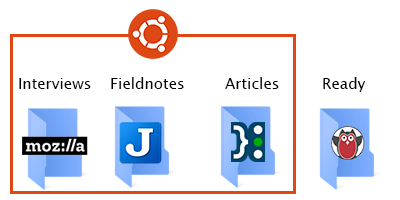
\includegraphics[width=1\textwidth,height=0.5\textheight,keepaspectratio]{%
figure/diagram.png}\\
\vspace{12pt}
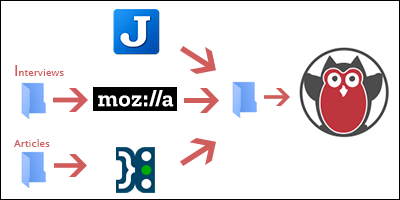
\includegraphics[width=1\textwidth,height=0.5\textheight,keepaspectratio]{%
figure/process.png}
    \end{column}
    \begin{column}[c]{0.45\textwidth}
    \parbox{\linewidth}{

1. Place audio files into the interviews folder and PDF files into the articles folder\\

2. Open Ubuntu and execute the script that transcribes audio with Mozilla Deepspeech, converts PDFs using xPDF, exports fieldnotes from Joplin, and places all files within the Ready folder\\

3. Open Voyant Server and select all files within Ready for analysis
      
      \vspace{12pt}
}
    \end{column}
    
  \end{columns}

  
\end{frame}

%%%%%%%%%%%%%%%%%%%%%%%%%%%%%%%%%%%%%%%%%%%%%%%%%%%%%%%%%%%%%%%%%%%%%%%%%%
\mysection{radar}
%%%%%%%%%%%%%%%%%%%%%%%%%%%%%%%%%%%%%%%%%%%%%%%%%%%%%%%%%%%%%%%%%%%%%%%%%%
\begin{frame}\label{\secvariable}
  \begin{columns}[t]
  %https://tex.stackexchange.com/a/7452/5483
    \begin{column}[c]{0.45\textwidth}
    \parbox{\linewidth}{

      \textbf{Mozilla's Project \\Deepspeech}\\
      is an open source Speech-To-Text engine, using a model trained by machine learning techniques based on Baidu's Deep Speech research paper. Project DeepSpeech uses Google's TensorFlow to make the implementation easier.\\
      It is only supported on Linux distributions.
      
      \vspace{12pt}
      
	  
      }
    \end{column}
    \begin{column}[c]{0.45\textwidth}
%http://lorempixel.com/1200/800/cats/Figure2/     
%http://lorempixel.com/1200/800/cats/Figure3/
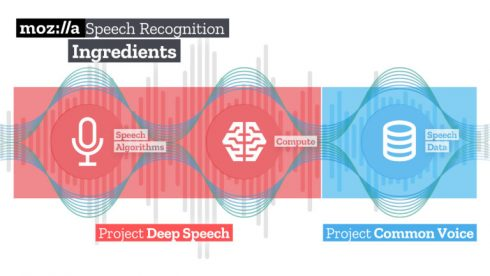
\includegraphics[width=1\textwidth,height=0.5\textheight,keepaspectratio]{%
figure/commonvoice.png}\\
\vspace{12pt}
More information can be found at \url{https://github.com/mozilla/DeepSpeech}
    \end{column}
  \end{columns}

  
\end{frame}

%%%%%%%%%%%%%%%%%%%%%%%%%%%%%%%%%%%%%%%%%%%%%%%%%%%%%%%%%%%%%%%%%%%%%%%%%%
\mysection{line}
%%%%%%%%%%%%%%%%%%%%%%%%%%%%%%%%%%%%%%%%%%%%%%%%%%%%%%%%%%%%%%%%%%%%%%%%%%
\begin{frame}\label{\secvariable}
\begin{center}
  \vspace{-0.5cm}
  %http://lorempixel.com/1200/800/cats/Figure4/
 
\includegraphics[width=1\textwidth,height=0.75\textheight,keepaspectratio]{%
  figure/Icon512.png}
\end{center}
  \vspace{-0.5cm}
  Joplin is an open source note taking and to-do application with synchronisation capabilities.

  $\quad \Rightarrow$ \url{https://joplinapp.org/}
  
\end{frame}

%%%%%%%%%%%%%%%%%%%%%%%%%%%%%%%%%%%%%%%%%%%%%%%%%%%%%%%%%%%%%%%%%%%%%%%%%%
\mysection{major}
%%%%%%%%%%%%%%%%%%%%%%%%%%%%%%%%%%%%%%%%%%%%%%%%%%%%%%%%%%%%%%%%%%%%%%%%%%
\begin{frame}\label{\secvariable} %%Eine Folie
\begin{center}
%http://lorempixel.com/1200/800/cats/Figure5/
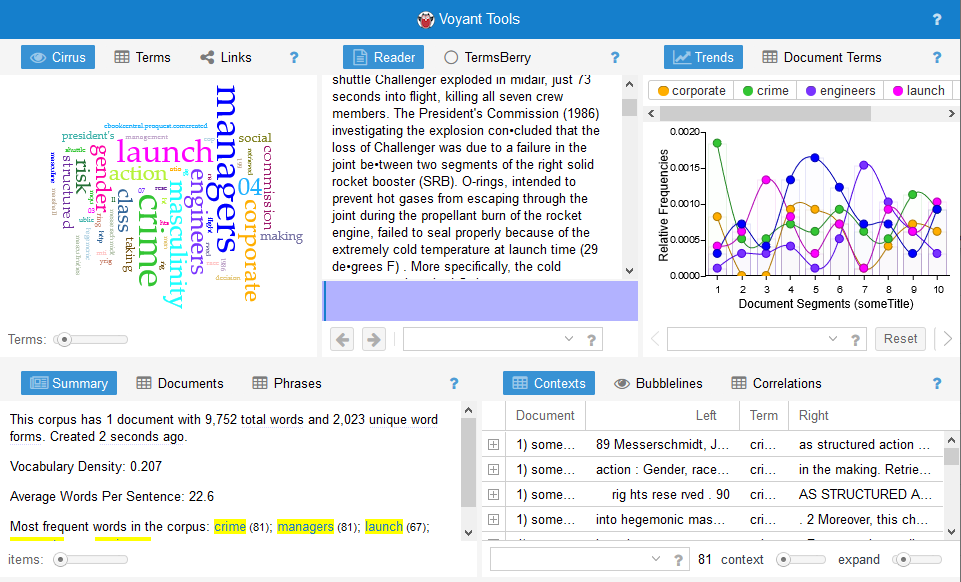
\includegraphics[width=1\textwidth,height=0.6\textheight,keepaspectratio]{%
figure/voyantuse.PNG}
\end{center}

    \parbox{\linewidth}{

Voyant is an open-source application for performing text analysis. It supports scholarly reading and interpretation of texts or corpus.\\
  $\quad \Rightarrow$ \url{http://docs.voyant-tools.org}
}
\end{frame}


%%%%%%%%%%%%%%%%%%%%%%%%%%%%%%%%%%%%%%%%%%%%%%%%%%%%%%%%%%%%%%%%%%%%%%%%%%
\mysection{conclusion}
%%%%%%%%%%%%%%%%%%%%%%%%%%%%%%%%%%%%%%%%%%%%%%%%%%%%%%%%%%%%%%%%%%%%%%%%%%
\begin{frame}\label{\secvariable}
  
 Additional information can be found in the following links:\\
 \url{https://github.com/MQ-FOAR705/HammondA_PoC_Design}
 \url{https://www.xpdfreader.com/pdftotext-man.html}
 \url{https://voyant-tools.org/}
 \url{https://github.com/mozilla/DeepSpeech}
 \url{https://joplinapp.org/}
  
\end{frame}



\end{document}
